\documentclass[12pt]{article}
\usepackage{authblk}
\usepackage{amsmath}
\usepackage{amssymb}
\usepackage{booktabs}
\usepackage{graphicx}
\usepackage{psfrag,epsf}
\usepackage{enumerate}
\usepackage{natbib}
\usepackage{url} % not crucial - just used below for the URL
\usepackage{comment}
\RequirePackage[colorlinks,citecolor=blue,urlcolor=blue]{hyperref}
\usepackage{setspace}

\newcommand{\jy}[1]{\textcolor{red}{JY: #1}}
\newcommand{\eds}[1]{\textcolor{blue}{(EDS: #1)}}
\newcommand{\mc}[1]{\textcolor{green}{(MC: #1)}}
\newcommand{\xz}[1]{\textcolor{cyan}{(XZ: #1)}}


\renewcommand{\thefigure}{S-\arabic{figure}}
\renewcommand{\thetable}{S-\arabic{table}}
\renewcommand{\thesection}{S-\arabic{section}}

\allowdisplaybreaks

\usepackage[pagewise]{lineno}
\linenumbers*[1]
% patches to make lineno work better with amsmath
\newcommand*\patchAmsMathEnvironmentForLineno[1]{%
        \expandafter\let\csname old#1\expandafter\endcsname\csname 
        #1\endcsname
        \expandafter\let\csname oldend#1\expandafter\endcsname\csname 
        end#1\endcsname
        \renewenvironment{#1}%
        {\linenomath\csname old#1\endcsname}%
        {\csname oldend#1\endcsname\endlinenomath}}%
\newcommand*\patchBothAmsMathEnvironmentsForLineno[1]{%
        \patchAmsMathEnvironmentForLineno{#1}%
        \patchAmsMathEnvironmentForLineno{#1*}}%
\AtBeginDocument{%
        \patchBothAmsMathEnvironmentsForLineno{equation}%
        \patchBothAmsMathEnvironmentsForLineno{align}%
        \patchBothAmsMathEnvironmentsForLineno{flalign}%
        \patchBothAmsMathEnvironmentsForLineno{alignat}%
        \patchBothAmsMathEnvironmentsForLineno{gather}%
        \patchBothAmsMathEnvironmentsForLineno{multline}%
}

\pdfminorversion=4
% NOTE: To produce blinded version, replace "0" with "1" below.
\newcommand{\blind}{0}

% DON'T change margins - should be 1 inch all around.
\addtolength{\oddsidemargin}{-.5in}%
\addtolength{\evensidemargin}{-.5in}%
\addtolength{\textwidth}{1in}%
\addtolength{\textheight}{1.3in}%
\addtolength{\topmargin}{-.8in}%


\begin{document}

%\bibliographystyle{natbib}

\def\spacingset#1{\renewcommand{\baselinestretch}%
{#1}\small\normalsize} \spacingset{1}


%%%%%%%%%%%%%%%%%%%%%%%%%%%%%%%%%%%%%%%%%%%%%%%%%%%%%%%%%%%%%%%%%%%%%%%%%%%%%%

\title{\bf Supplementary Material to\\
  ``Nonparametric Block Bootstrap Kolmogorov-Smirnov Goodness-of-Fit Test''
}
\if0\blind
{
  \author[1,2]{Mathew Chandy}
  \author[1]{Elizabeth D. Schifano}
  \author[1]{Jun Yan\thanks{
    The authors gratefully acknowledge the National Science Foundation (NSF).}\hspace{.2cm}}
  \author[3]{Xianyang Zhang$^{\ast}$ }
  \affil[1]{Department of Statistics, University of Connecticut}
  \affil[2]{Department of Statistics and Data Science, University of California, Los Angeles}
  \affil[3]{Department of Statistics, Texas A\&M University}
  \maketitle
} \fi

\if1\blind
{
  \bigskip
  \bigskip
  \bigskip
  \author{Anonymous Author}
} \fi

\maketitle

\section{Comparison of Two Bias Corrections}

\begin{figure}[tbp]
  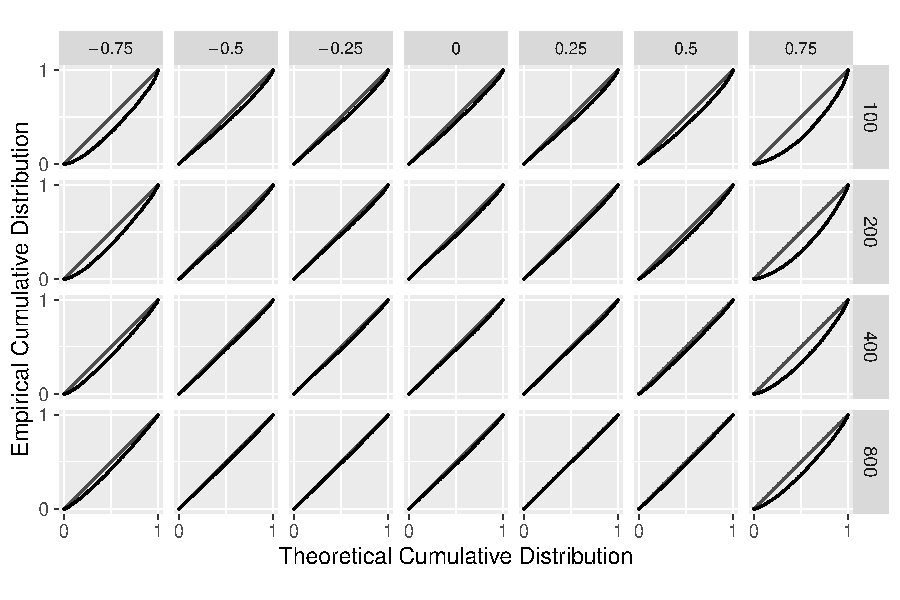
\includegraphics[width = .9\textwidth]{figures/normal_C_n}
  \centering
  \vspace{-10pt}
  \caption{Q-Q plots of the p-values testing that a time series
    has a marginal Normal distribution with true data generating distribution
    being $N(8,8)$ when using  bias correction term $C_n$.}
  \label{fig:qq_n_C_n}
    \hspace{3cm}
  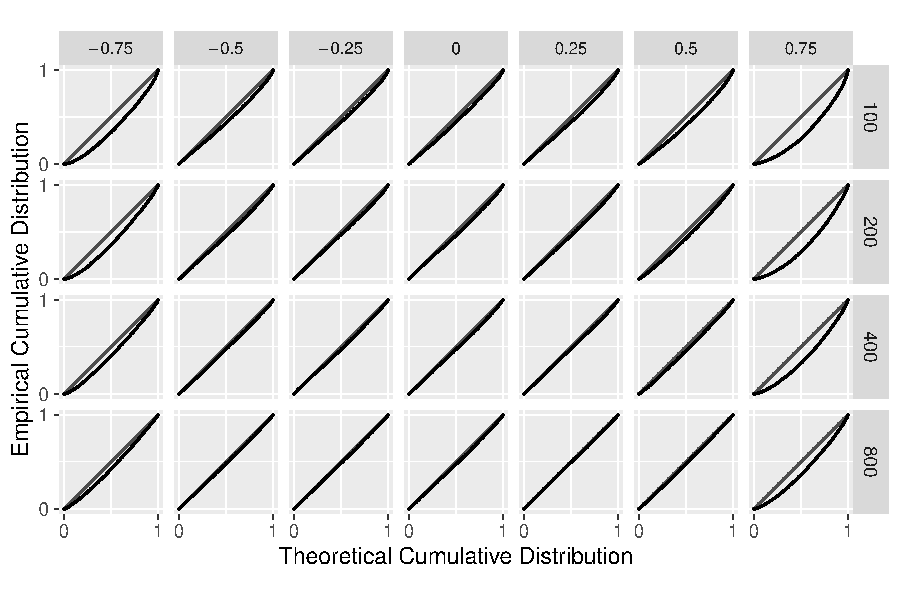
\includegraphics[width = .9\textwidth]{figures/gamma_C_n}
  \vspace{-5pt}
  \caption{Q-Q plots of the p-values testing that a time series
    has a marginal Gamma distribution with true data generating distribution
    being $\Gamma(8,1)$ when using  bias correction term $C_n$.}
  \label{fig:qq_g_C_n}
\end{figure}


\begin{figure}[tbp]
  \centering
  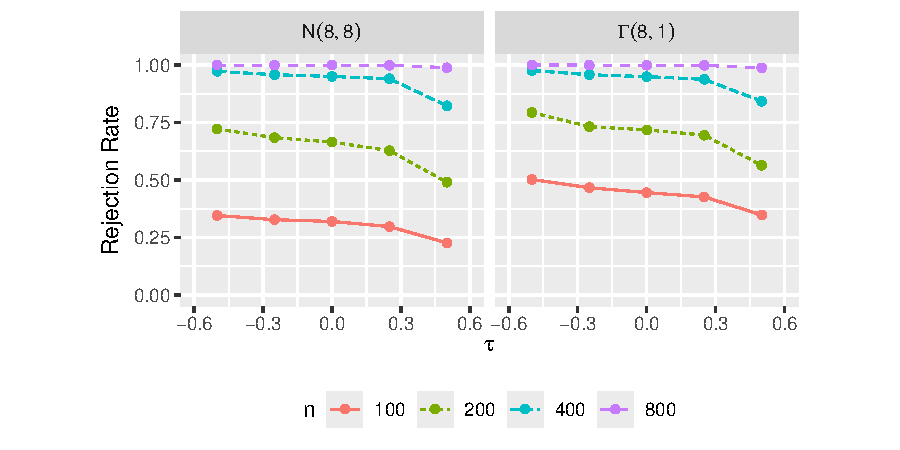
\includegraphics[scale=1]{figures/rr_C_n}
  \caption{Empirical power curve as a function of $\tau$ for
    $n \in \{100, 200, 400, 800\}$ and true marginal distribution
    $\in \{N(8,8), \Gamma(8,1)\}$, when using bias correction term
    $C_n$. When the data was generated from $N(8,8)$,
    we tested for the Gamma family. When the data was generated from
    $\Gamma(8,1)$, we tested for the Normal family.
  }
  \label{fig:rr_C_n}
\end{figure}


To evaluate the practical difference between the two bias correction
terms, this section presents a direct comparison between the
nonparametric block bootstrap KS tests based on $K_n(x)$ and on
$C_n(x)$. The $K_n(x)$ correction, which was heuristically justified in
the main manuscript, is designed to center the empirical process in a
manner consistent with the dependence structure of the series. In
contrast, $C_n(x)$ is the bias correction proposed by
\citet{babu2004goodness} for independent observations.


A simulation study was conducted using the same settings as in the main
paper, varying sample size, block length, and dependence strength, with
the only difference being the choice of bias correction term.
Figures~\ref{fig:qq_n_C_n}--\ref{fig:rr_C_n} present the results for
$C_n(x)$, which are the counterparts of the figures in the main
manuscript obtained
using $K_n(x)$. Across the same parameter configurations, both versions
of the test maintain comparable size and power, and their performance
differences appear negligible for the cases examined.


These findings suggest that, within the range of settings studied, the
circular block bootstrap already removes most dependence-induced bias,
so that the additional centering adjustment has limited practical
impact. Although $C_n(x)$ requires slightly less computation, we
continue to recommend $K_n(x)$ for its theoretical motivation, while
recognizing that in the present experiments their empirical behavior is
essentially indistinguishable.


\section{Block Size Selection}


\begin{figure}[tbp]
  \centering
  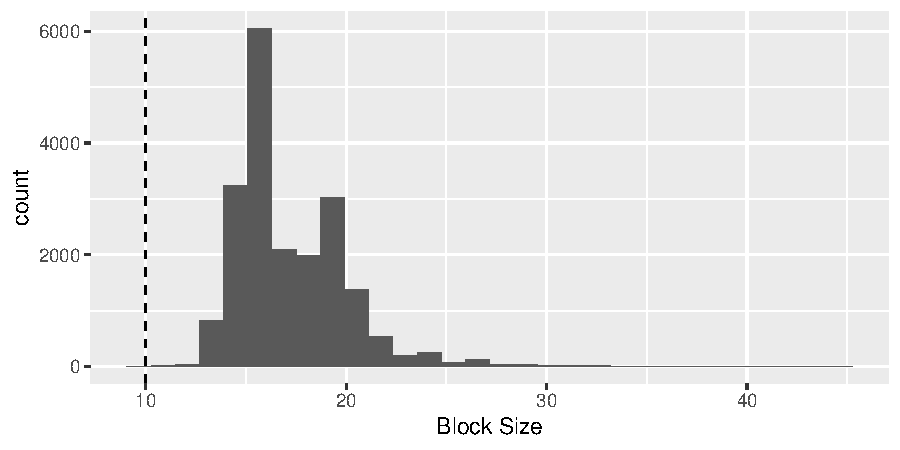
\includegraphics[scale=1]{figures/block_dist}
  \caption{Distribution of the selected block sizes using
    \citet{politis2004automatic}'s procedure applied to 20,000
    time series of length-800 with
    Kendall's $\tau = 0.5$ data generating distribution $N(8,8)$. The vertical
    dashed line marks $l = \lceil n^{1/3} \rceil \approx 10$.
  }
  \label{fig:block_dist}
% \end{figure}


% \begin{figure}[tbp]
  \centering
  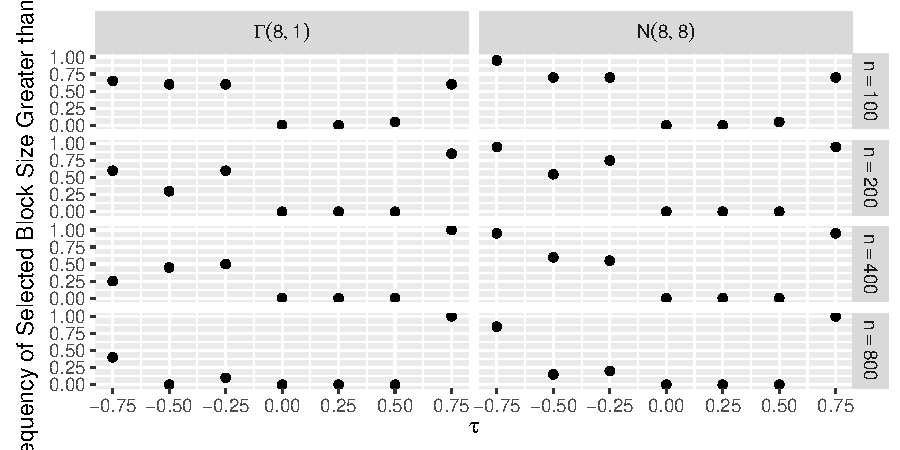
\includegraphics[scale=1]{figures/large_block}
  \caption{Proportion of selected block sizes using the method of
  \citet{politis2004automatic} that are larger than
    $\sqrt{n}$ for $n \in \{100, 200, 400, 800\}$,
    $\tau \in \{-0.75, -0.50, -0.25, 0, 0.25, 0.50, 0.75\}$, and true
    marginal distribution $N(8,8)$ and $\Gamma(8,1)$.
  }
  \label{fig:large_block}
\end{figure}

The choice of block size plays a central role in determining the
finite-sample behavior of block bootstrap methods when serial
dependence is present. Although our main simulations used the fixed rule
$l = \lceil n^{1/3} \rceil$, the effective block size can vary with the
strength and pattern of dependence
\citep{hall1995blocking, buhlmann1999block, politis2004automatic}.
To evaluate the impact of data-driven selection, we examined the
automatic block-length procedure proposed by
\citet{politis2004automatic}, which selects the block size adaptively
from the observed series. All other simulation settings were kept
identical to those in the main paper.


The automatically selected block sizes were generally larger than the
fixed choice $l = \lceil n^{1/3} \rceil$, as anticipated, but the
procedure sometimes produced unrealistically large values under certain
dependence structures. In particular, when the series exhibited strong
negative or very strong positive dependence, the selected block sizes
were often excessively large---occasionally comparable to or exceeding
the sample size $n$. In our implementation, we set the final block
length to $\min\{n, \hat{l}\}$, where $\hat{l}$ denotes the value
returned by the automatic procedure. Figure~\ref{fig:block_dist}
illustrates the typical distribution of selected block sizes for $n =
800$, $\tau = 0.5$, and $X_i \sim N(8,8)$, showing that most values
exceed $\lceil n^{1/3} \rceil$ and many approach or surpass
$\sqrt{n}$. Figure~\ref{fig:large_block} further summarizes the
proportion of selected block sizes greater than $\sqrt{n}$ across
different dependence levels and sample sizes, indicating that such
oversizing occurs systematically under strong negative and very strong
positive dependence.


\begin{figure}[tbp]
  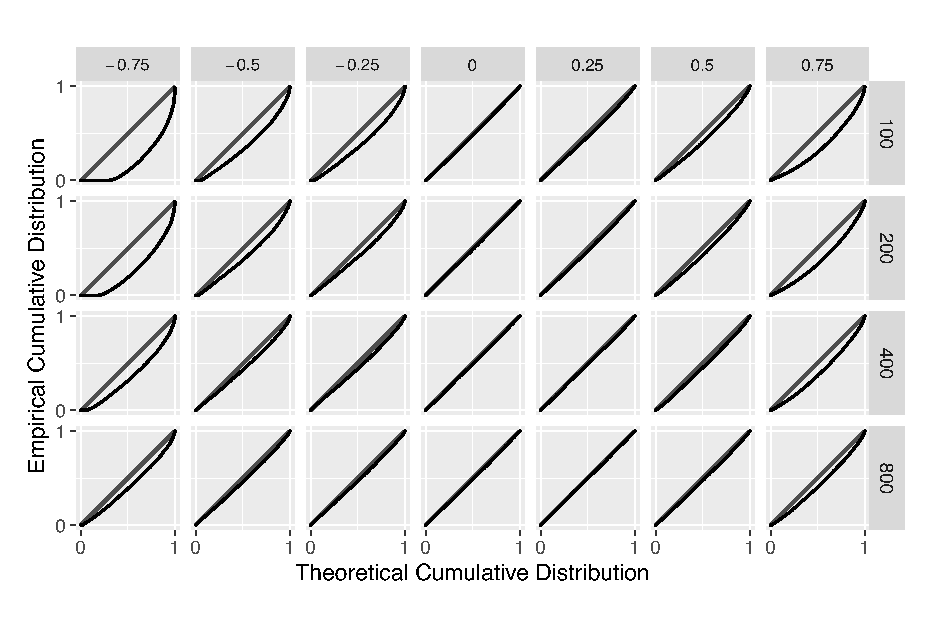
\includegraphics[width = .9\textwidth]{figures/alt_normal}
  \centering
  \vspace{-10pt}
  \caption{Q-Q plots of the p-values testing that a time series
    has a marginal Normal distribution with true data generating distribution
    being $N(8,8)$, when using \citet{politis2004automatic}'s procedure
    to select block sizes.}
  \label{fig:alt_qq_n}
    \hspace{3cm}
  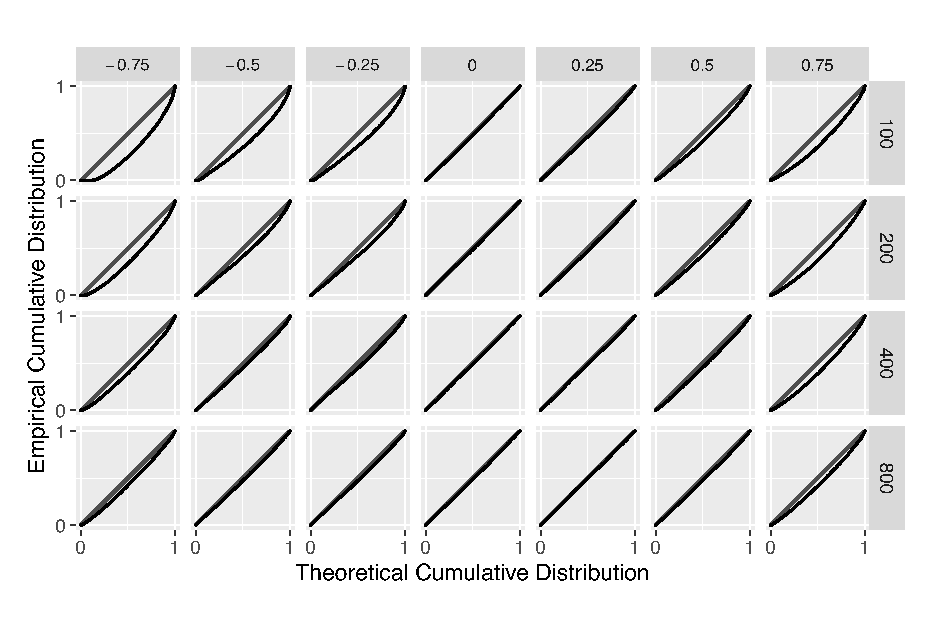
\includegraphics[width = .9\textwidth]{figures/alt_gamma}
  \vspace{-5pt}
  \caption{Q-Q plots of the p-values testing that a time series
    has a marginal Gamma distribution with true data generating distribution
    being $\Gamma(8,1)$, when using \citet{politis2004automatic}'s procedure
    to select block sizes.}
  \label{fig:alt_qq_g}
\end{figure}


\begin{figure}[tbp]
  \centering
  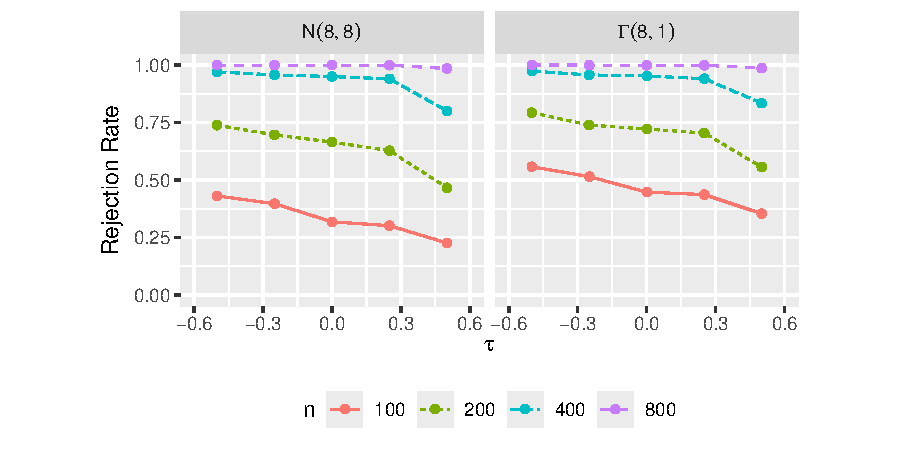
\includegraphics[scale=1]{figures/alt_rr}
  \caption{Empirical power curve as a function of $\tau$ for
    $n \in \{100, 200, 400, 800\}$ and true marginal distribution
    $\in \{N(8,8), \Gamma(8,1)\}$, when using \citet{politis2004automatic}'s 
    procedure
    to select block sizes. When the data was generated from $N(8,8)$,
    we tested for the Gamma family. When the data was generated from
    $\Gamma(8,1)$, we tested for the Normal family.
  }
  \label{fig:alt_rr}
\end{figure}


We next evaluated the size and power performance of the NPBB test when
the block length was chosen automatically.
Figures~\ref{fig:alt_qq_n} and~\ref{fig:alt_qq_g} display the empirical
size through Q--Q plots of the $p$-values under the null for Normal and
Gamma margins, respectively. For reference, the main paper showed that
the fixed cubic root rule $l = \lceil n^{1/3} \rceil$ maintained size
reasonably well for small~$n$ when $|\tau| \le 0.25$, whereas achieving
nominal size required $n > 200$ for $|\tau| \ge 0.5$ and $n > 800$ for
$|\tau| \ge 0.75$. The automatic selection exhibits a similar pattern
of limitations: for $|\tau| > 0.5$, the empirical size again departs
from nominal levels. Deviations from the diagonal line are more
pronounced for negative~$\tau$, consistent with the high frequency of
excessively large block sizes in those cases. For instance, while the
cubic root rule held size adequately at $\tau = -0.25$ with small~$n$,
the automatic procedure no longer does. In contrast, for
$\tau \in \{0, 0.25\}$, the automatically selected block sizes yield
size control comparable to the fixed rule, indicating satisfactory
performance for weak or moderate positive dependence.


Figure~\ref{fig:alt_rr} summarizes the power analysis under automatic
selection. Relative to the main paper’s results based on the cubic root
rule, the two approaches show broadly similar power for
$|\tau| \le 0.5$, with the automatic method occasionally achieving
slightly higher rejection rates for small samples with mild negative
dependence. Overall, these findings indicate that the automatic
procedure of \citet{politis2004automatic} performs reasonably well under
most conditions studied but may yield unstable results when dependence
is negative and sample sizes are small. In such cases, it is advisable
to adopt a more restrictive cap on the final block size---for example,
setting it to $\min\{\sqrt{n}, \hat{l}\}$---to avoid excessive block
lengths that can distort the bootstrap resampling.


\bibliographystyle{asa}
\bibliography{citations}
\end{document}
